\documentclass[11pt]{article}

\usepackage{latexsym}
\usepackage{amsmath}
\usepackage{amssymb}
\usepackage{amsthm}
\usepackage{graphicx}
\usepackage{wrapfig}
\usepackage{pseudocode}
\usepackage{url}
\usepackage[backref, colorlinks=true, citecolor=red, urlcolor=blue, pdfauthor={Jyh-Ming Lien}]{hyperref}
\usepackage{subfigure}

\newcommand{\handout}[5]{
  \noindent
  \begin{center}
  \framebox{
    \vbox{
      \hbox to 5.78in { {\bf } \hfill #2 }
      \vspace{4mm}
      \hbox to 5.78in { {\Large \hfill #5  \hfill} }
      \vspace{2mm}
      \hbox to 5.78in { {\em #3 \hfill #4} }
    }
  }
  \end{center}
  \vspace*{4mm}
}

\newcommand{\lecture}[4]{\handout{#1}{#2}{#3}{}{Report for #1}}

\newtheorem{theorem}{Theorem}
\newtheorem{corollary}[theorem]{Corollary}
\newtheorem{lemma}[theorem]{Lemma}
\newtheorem{observation}[theorem]{Observation}
\newtheorem{proposition}[theorem]{Proposition}
\newtheorem{definition}[theorem]{Definition}
\newtheorem{claim}[theorem]{Claim}
\newtheorem{fact}[theorem]{Fact}
\newtheorem{assumption}[theorem]{Assumption}

% 1-inch margins, from fullpage.sty by H.Partl, Version 2, Dec. 15, 1988.
\topmargin 0pt
\advance \topmargin by -\headheight
\advance \topmargin by -\headsep
\textheight 8.9in
\oddsidemargin 0pt
\evensidemargin \oddsidemargin
\marginparwidth 0.5in
\textwidth 6.5in

\parindent 0in
\parskip 1.5ex
%\renewcommand{\baselinestretch}{1.25}

\begin{document}

\lecture{Advance Algorithm Programming Assignment 1 }{Fall 2015}{Youngeun Lee}{---}


\section{Implementation Details}

The goal of this assignment is to implement $\alpha$-shape for a given value of $\alpha$. Tetrahedrons in the Delaunay triangulation computed using the previous assignment. The program get the center of circumspheres of the tetragedrons by $qh_facetcenter()$ function in qhull. The center are computed in 4D then computed in 3D.

\section{Example Output}

Fig.~\ref{fig:bb}, \ref{fig:bull}, \ref{fig:bunny}, \ref{fig:cube}, \ref{fig:ellipsoid}, \ref{fig:screwdriver}, \ref{fig:spoon}, \ref{fig:T}, \ref{fig:teeth}, \ref{fig:U}, \ref{fig:woman} and \ref{fig:Y} show results of each test file. (a) in the figures show their Delaunay triangulation and (b)-(d) present $\alpha$-shape with different values.

\begin{figure}[!htb]
\centering
\subfigure[Delaunay triangulation]{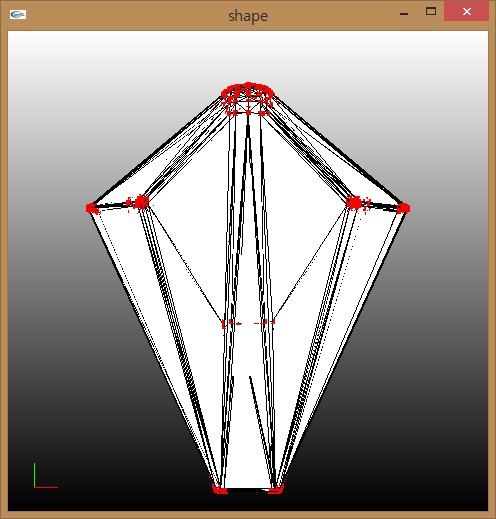
\includegraphics[height=4.0cm]{./figs/bb_t.jpg}}
\subfigure[$\alpha=150$]{\includegraphics[height=4.0cm]{./figs/bb_50.jpg}}
\subfigure[$\alpha=100$]{\includegraphics[height=4.0cm]{./figs/bb_100.jpg}}
\subfigure[$\alpha=50$]{\includegraphics[height=4.0cm]{./figs/bb_150.jpg}}
\caption{i.bb}
\label{fig:bb}
\end{figure}

\begin{figure}[!htb]
\centering
\subfigure[Delaunay triangulation]{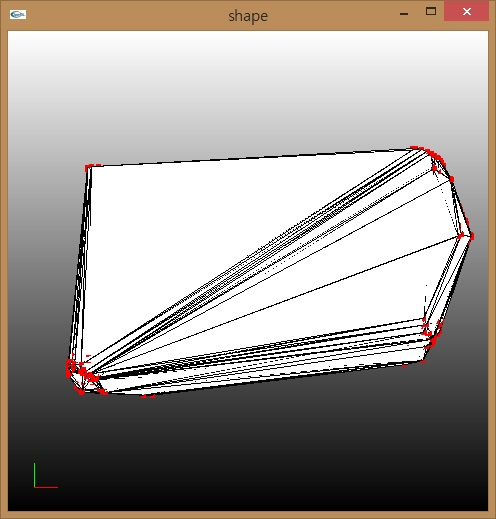
\includegraphics[height=4.0cm]{./figs/bull_t.jpg}}
\subfigure[$\alpha=10^6$]{\includegraphics[height=4.0cm]{./figs/bull_1000000.jpg}}
\subfigure[$\alpha=5\*10^5$]{\includegraphics[height=4.0cm]{./figs/bull_500000.jpg}}
\subfigure[$\alpha=10^5$]{\includegraphics[height=4.0cm]{./figs/bull_100000.jpg}}
\caption{i.bull}
\label{fig:bull}
\end{figure}

\begin{figure}[!htb]
\centering
\subfigure[Delaunay triangulation]{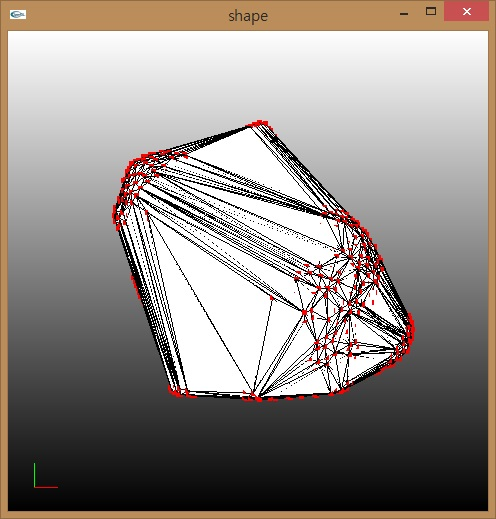
\includegraphics[height=4.0cm]{./figs/bunny_t.jpg}}
\subfigure[$\alpha=10^5$]{\includegraphics[height=4.0cm]{./figs/bunny_100000.jpg}}
\subfigure[$\alpha=10^4$]{\includegraphics[height=4.0cm]{./figs/bunny_10000.jpg}}
\subfigure[$\alpha=10^3$]{\includegraphics[height=4.0cm]{./figs/bunny_1000.jpg}}
\caption{i.bunny}
\label{fig:bunny}
\end{figure}

\begin{figure}[!htb]
\centering
\subfigure[Delaunay triangulation]{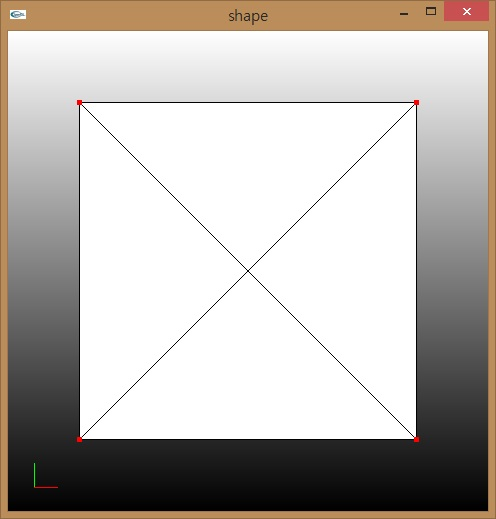
\includegraphics[height=4.0cm]{./figs/cube_t.jpg}}
\subfigure[$\alpha=76$]{\includegraphics[height=4.0cm]{./figs/cube_76.jpg}}
\subfigure[$\alpha=75$]{\includegraphics[height=4.0cm]{./figs/cube_75.jpg}}
\subfigure[$\alpha=74$]{\includegraphics[height=4.0cm]{./figs/cube_74.jpg}}
\caption{i.cube}
\label{fig:cube}
\end{figure}

\begin{figure}[!htb]
\centering
\subfigure[Delaunay triangulation]{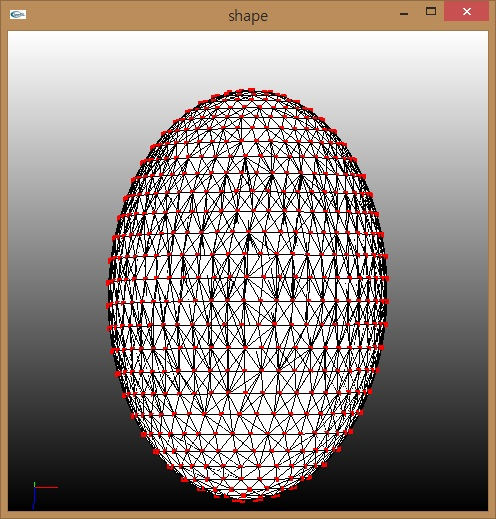
\includegraphics[height=4.0cm]{./figs/ellipsoid_t.jpg}}
\subfigure[$\alpha=20000$]{\includegraphics[height=4.0cm]{./figs/ellipsoid_20000.jpg}}
\subfigure[$\alpha=10000$]{\includegraphics[height=4.0cm]{./figs/ellipsoid_10000.jpg}}
\subfigure[$\alpha=5000$]{\includegraphics[height=4.0cm]{./figs/ellipsoid_5000.jpg}}
\caption{i.ellipsoid}
\label{fig:ellipsoid}
\end{figure}

\begin{figure}[!htb]
\centering
\subfigure[Delaunay triangulation]{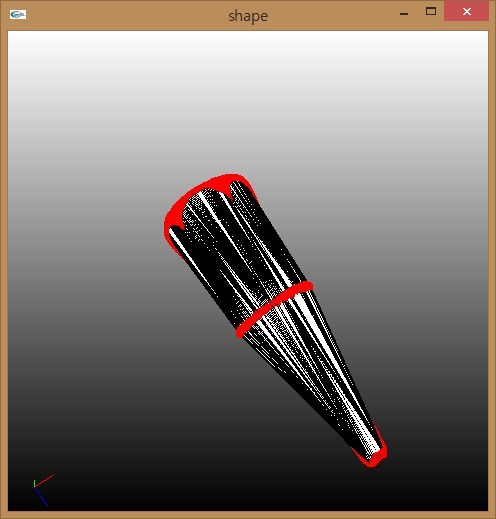
\includegraphics[height=4.0cm]{./figs/screwdriver_t.jpg}}
\subfigure[$\alpha=10^7$]{\includegraphics[height=4.0cm]{./figs/screwdriver_10000000.jpg}}
\subfigure[$\alpha=10^6$]{\includegraphics[height=4.0cm]{./figs/screwdriver_1000000.jpg}}
\subfigure[$\alpha=10^5$]{\includegraphics[height=4.0cm]{./figs/screwdriver_100000.jpg}}
\caption{i.screwdriver}
\label{fig:screwdriver}
\end{figure}

\begin{figure}[!htb]
\centering
\subfigure[Delaunay triangulation]{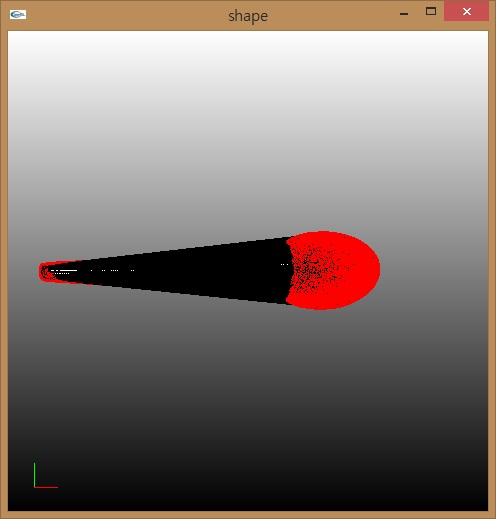
\includegraphics[height=4.0cm]{./figs/spoon_t.jpg}}
\subfigure[$\alpha=10^8$]{\includegraphics[height=4.0cm]{./figs/spoon_100000000.jpg}}
\subfigure[$\alpha=10^7$]{\includegraphics[height=4.0cm]{./figs/spoon_10000000.jpg}}
\subfigure[$\alpha=10^6$]{\includegraphics[height=4.0cm]{./figs/spoon_1000000.jpg}}
\caption{i.spoon}
\label{fig:spoon}
\end{figure}

\begin{figure}[!htb]
\centering
\subfigure[Delaunay triangulation]{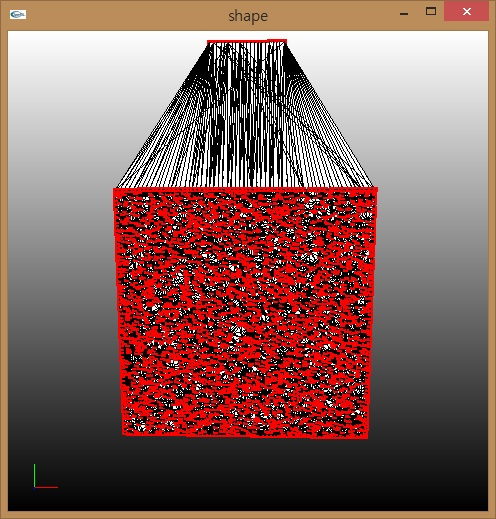
\includegraphics[height=4.0cm]{./figs/T_t.jpg}}
\subfigure[$\alpha=10000$]{\includegraphics[height=4.0cm]{./figs/T_10000.jpg}}
\subfigure[$\alpha=1000$]{\includegraphics[height=4.0cm]{./figs/T_1000.jpg}}
\subfigure[$\alpha=100$]{\includegraphics[height=4.0cm]{./figs/T_100.jpg}}
\caption{i.T}
\label{fig:T}
\end{figure}

\begin{figure}[!htb]
\centering
\subfigure[Delaunay triangulation]{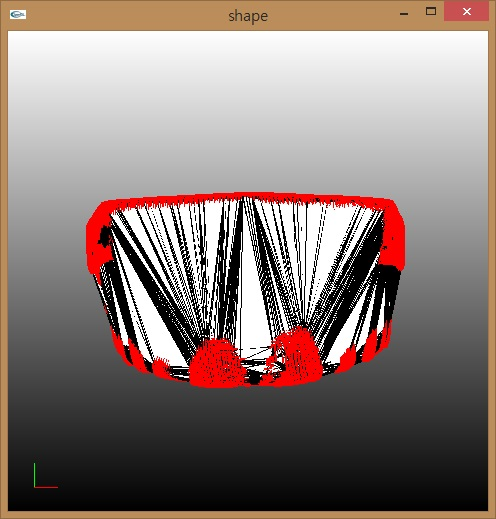
\includegraphics[height=4.0cm]{./figs/teeth_t.jpg}}
\subfigure[$\alpha=100000$]{\includegraphics[height=4.0cm]{./figs/teeth_100000.jpg}}
\subfigure[$\alpha=10000$]{\includegraphics[height=4.0cm]{./figs/teeth_10000.jpg}}
\subfigure[$\alpha=1000$]{\includegraphics[height=4.0cm]{./figs/teeth_1000.jpg}}
\caption{i.teeth}
\label{fig:teeth}
\end{figure}

\begin{figure}[!htb]
\centering
\subfigure[Delaunay triangulation]{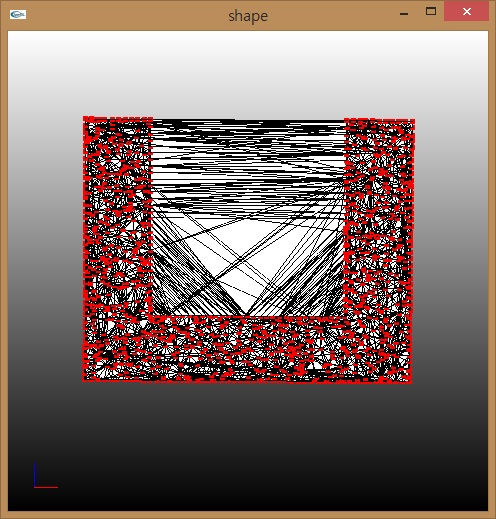
\includegraphics[height=4.0cm]{./figs/U_t.jpg}}
\subfigure[$\alpha=10000$]{\includegraphics[height=4.0cm]{./figs/U_10000.jpg}}
\subfigure[$\alpha=1000$]{\includegraphics[height=4.0cm]{./figs/U_1000.jpg}}
\subfigure[$\alpha=100$]{\includegraphics[height=4.0cm]{./figs/U_100.jpg}}
\caption{i.U}
\label{fig:U}
\end{figure}

\begin{figure}[!htb]
\centering
\subfigure[Delaunay triangulation]{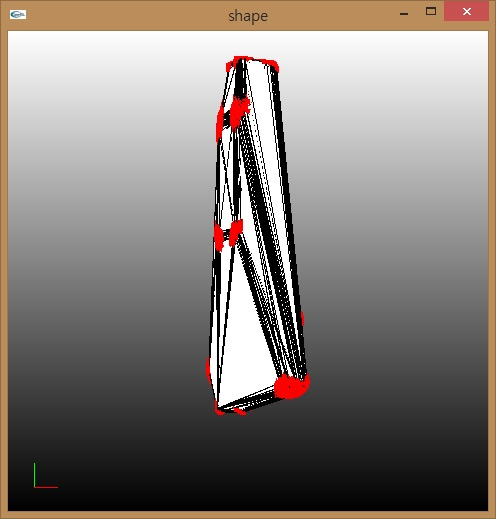
\includegraphics[height=4.0cm]{./figs/woman_t.jpg}}
\subfigure[$\alpha=100000$]{\includegraphics[height=4.0cm]{./figs/woman_100000.jpg}}
\subfigure[$\alpha=10000$]{\includegraphics[height=4.0cm]{./figs/woman_10000.jpg}}
\subfigure[$\alpha=1000$]{\includegraphics[height=4.0cm]{./figs/woman_1000.jpg}}
\caption{i.woman}
\label{fig:woman}
\end{figure}

\begin{figure}[!htb]
\centering
\subfigure[Delaunay triangulation]{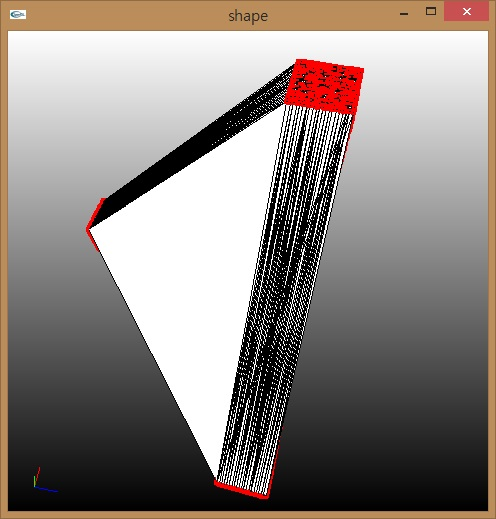
\includegraphics[height=4.0cm]{./figs/Y_t.jpg}}
\subfigure[$\alpha=100000$]{\includegraphics[height=4.0cm]{./figs/Y_100000.jpg}}
\subfigure[$\alpha=10000$]{\includegraphics[height=4.0cm]{./figs/Y_10000.jpg}}
\subfigure[$\alpha=1000$]{\includegraphics[height=4.0cm]{./figs/Y_1000.jpg}}
\caption{i.Y}
\label{fig:Y}
\end{figure}

\section{Know bugs/limitations}

$\alpha$-shape can compute more precise surfaces from the given points than Delaunay triangulation. However, if a point set is not dense enough, it makes holes.

%\bibliographystyle{plain}
%\bibliography{report}

\end{document}


